\chapter{Project Progress}\label{ch:progress}

Previously in thesis A we elected Minigent as the place to design our new recursive types for Cogent.
Our design was to introduce a new recursive parameter to Minigent's boxed records, in order to allow
for recursively nested data structures. These data structures would be strictly positive as per
definition \autoref{def:sp}, to prevent the programmer constructing infinitely recursive
objects that would lead to termination issues, thus allowing for ease of verification in
the Isabelle embedding.

Work has been completed to incorporate the design into the parser, lexer and reorganiser compiler phases of
Minigent, and work has begun work on integrating updatin the type checking phase.
In addition to the existing suite of tests in the Minigent compiler, additional tests have 
been added to test the newly added extension.

\todo{I'm starting to think this isn't very relevant to the thesis report, let alone the project. Remove?} \\
In order to increase my work efficiency, I created an extension in VSCode that provides syntax highlighting
for both Cogent and Minigent files, which allowed for an easier experience when constructing Minigent programs,
and hence made it easier to write tests for new features.

My work has progressed according to my thesis A schedule, as in \autoref{fig:thesisATimeline}. However, due to 
new discoveries \todo{$<$- rephrase that } for the work on the type checker, my plan has changed for 
thesis C to allow more time for extensions, which are outlined in \autoref{ch:plan}.

\section{Parser and Lexer}

The Minigent lexer and parser now accepts a new recursive parameter extension to boxed records,
as seen in \autoref{fig:recursiveParameter}.

\begin{figure}
    \centering
    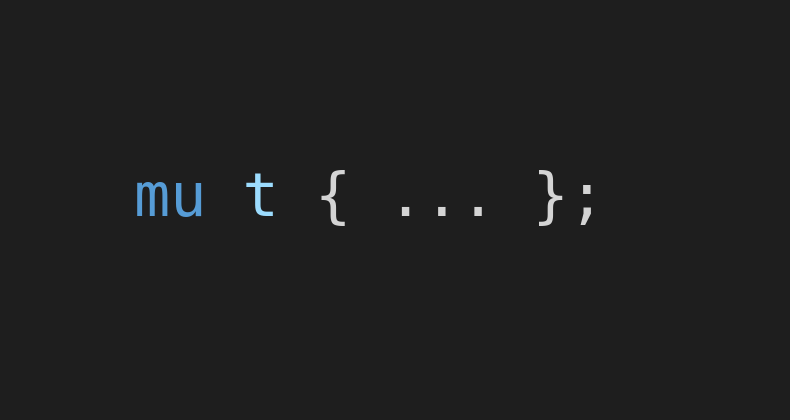
\includegraphics[width=0.5\linewidth]{content/recursive_parameter.png}
    \caption{The new recursive parameter grammar for boxed records}
    \label{fig:recursiveParameter}
\end{figure}

This new syntax is backwards compatible with the previous record syntax, so records without this new
syntax in old code will not have to be changed in order for the change to be implemented.

\todo{Should I talk about the code I wrote here?}

\section{Reorganiser}

In the reorganiser, a strict positivity check has been added to prevent the construction of infinitely
recursive objects. This check recursively evaluates all of the functions in a Minigent program, and
checks that their types do not contain a non-strictly positve type. This check also accounts for the
shadowing of recursive parameter variables, in the event a nested boxed record declaration's recursive
parameter shadows the parent record's parameter. These new recursive parameters are now distinguished from
regular type variables, and the reorganiser no longer counts them as type variables.

Functions that also call themselves successfully typecheck as their type signature provides enough information
to check the argument passed to the function, so basic recursion works as expected.

\todo{Unused recursive parameter variables?}

\section{Type Checker}

Work has begun on the type checker to check the types of records.

\todo{Talk about the stuff}

\section{Testing}

A suite of tests has been added to the existing Minigent test suite in order to test the new extension's 
expected behaviour.

The tests aim to test the intended functionality of our recursive types, including constructing and manipulating
recursive data structures (such as lists), as well as recursive functions that do not use our recursive types 
(such as functions recursing on U32 integers, etc.).

An example of such a test is seen in \autoref{fig:test1}, which constructs an empty list given the presence of an external allocation function.

\begin{figure}
    \centering
    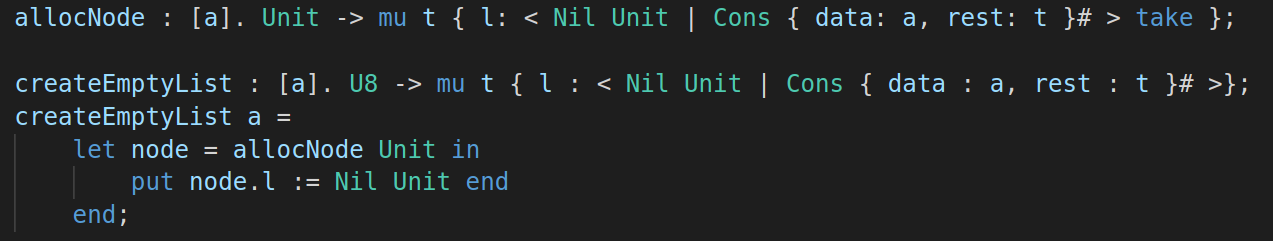
\includegraphics[width=\linewidth]{content/test1.png}
    \caption{Testing the construction of an empty list}
    \label{fig:test1}
\end{figure}

These tests also test the intended effects of our new types, such as the strict positivity guarantee they provide
and their interaction with the existing type system. Whilst the existing tests test the backwards compatability of
record types, our new tests check that no recursive parameters are used non-strictly positive, that shadowing of recursive
parameters behaves as intended, and that recursive parameters are seperate from quantified type variables.

\todo{talk about sp testing and such}

\section{Work efficiency}

\todo{talk about syntax highlighting, but also potentially remove}
